%%% Preamble
\documentclass[paper=a4, fontsize=12pt]{scrartcl}	
\usepackage[utf8]{inputenc}
\usepackage{tgbonum}
\usepackage[T1]{fontenc}
\usepackage{fourier}
\usepackage{setspace}
\usepackage[english]{babel}		% English language/hyphenation
\usepackage[protrusion=true,expansion=true]{microtype}				% Better typography
\usepackage{amsmath,amsfonts,amsthm}										% Math packages
\usepackage[pdftex]{graphicx}														% Enable pdflatex
\usepackage{url}
\usepackage{multirow}
\usepackage{color}
\usepackage{float}

%%% Custom sectioning (sectsty package)
\usepackage{sectsty}												% Custom sectioning (see below)
\allsectionsfont{\centering \normalfont\scshape}	% Change font of al section commands


%%% Custom headers/footers (fancyhdr package)
\usepackage{fancyhdr}
\pagestyle{fancyplain}
\fancyhead{}														% No page header
\fancyfoot[L]{}		% You may remove/edit this line 
\fancyfoot[C]{}													% Empty
\fancyfoot[R]{\thepage}									% Pagenumbering
\renewcommand{\headrulewidth}{0pt}			% Remove header underlines
\renewcommand{\footrulewidth}{0pt}				% Remove footer underlines
\setlength{\headheight}{0pt}


%%% Equation and float numbering
\numberwithin{equation}{section}		
\numberwithin{figure}{section}			
\numberwithin{table}{section}				


%%% Maketitle metadata
\newcommand{\horrule}[1]{\rule{\linewidth}{#1}} 	% Horizontal rule

\usepackage{amsmath, bbm}
\newcommand{\argmax}[1]{\underset{#1}{\operatorname{arg}\,\operatorname{max}}\;}
\newcommand{\argmin}[1]{\underset{#1}{\operatorname{arg}\,\operatorname{min}}\;}


\title{
		%\vspace{-1in} 	
		\usefont{OT1}{bch}{b}{n}
		\normalfont \normalsize \textsc{STAT 591: Adv Topics in Statistics} \\ [10pt]
		\huge Report of Using Generalized Correlation to effect Variable Selection in Very High Dimensional Problems \\
}
\author{
		\normalfont 								\normalsize
        Xuelong Wang \\[-3pt]		\normalsize
        \today
}
\date{}


%%% Begin document
\begin{document}
\maketitle
\section{Abstract}
\singlespacing
Under the linear assumption, many variable selection methods are able to work well. In other circumstances, nonlinearity of response can result in significant vector components being overlooked (important variables are not selected). Even if good results are obtained by linear model fitting, they can sometimes be bettered by using a nonlinear approach. These circumstances can arise in practice, with real data, and they motivate alternative methodologies. The authors of this paper suggest an approach based on ranking generalized empirical correlations between the response variable and components of the explanatory vector. This technique is not prediction-based, and can identify variables that are influential but not explicitly part of a predictive model. I will briefly introduce the problem they define and the solution for that particular problem, following by some simulation results and conclusion. 

\section{Problem trying to solve}
\subsection{Introduction}
\textit{\textbf{Traditional linear assumption}}: A variety of linear model-based methods have been proposed for variable selection. In this approach it is argued that a response variable, Yi , might be expressible as a linear form in a long p-vector, Xi , of explanatory variables, plus error, that is,

\[
  Y_i = \alpha + \beta_1X_{i1} + \dots + \beta_{p}X_{ip} + error
\]
and the variable selection can be achieved by choosing many of the coefficients $\beta_i's$ to be zero. Lasso is one of variable selection methods which is popular and effective. \\

\textit{\textbf{What if the linear assumption does not hold ?}}: The authors has shown that there will be risks for fitting a wrong linear model. When the underline model is non-linear, using the linear model may cause one to overlook some important components altogether. Following is an example.\\

\textit{\textbf{The Collinearity problem}}: Although the true model is linear, collinearity may conceal components that potentially influence linearly the value of $Y_i$. For instance, genes whose expression levels are strongly linearly associated with $Y_i$ , and so would be of biological interest, can be confounded or not uniquely represented. In particular, if $X_{i1} = X_{i3} +X_{i4}$ and $X_{i2} = X_{i3} +X_{i5}$, then the linear models $Y_i = X_{i1} - X_{i2} +error$ and $Yi = X_{i4} - X_{i5} +error$, and of course infinitely many others, are equally valid. This non-identifiability issue arises because the variable-selection problem is posed as one of model fitting, or prediction, which in our view is not necessarily a good idea. 

\subsection{Motivating Examples}
The authors have provided several motivation examples for supporting their point of view for the model-based variable selection methods. I only pick the example 2 for this report.

\textit{\textbf{Example 2, Acute leukemia microarray data}}: These data come from a study by Golub et al. (1999), where the aim was to use microarray evidence to distinguish between two types of acute leukemia (ALL/AML). There were p = 7,129 genes and n = 38 observations in the training data (27 ALL and 11 AML). 

\textit{\textbf{Interesting results}}: This dataset had been studied by previous paper, in which some model-based linear models were used for variable selection. According to their results, there was a gene called Msa.2877 which was selected as an important variable and had a strong correlation with response y. However, after the authors test the non-linear relation of components of x and y, they find another gene names Msa.11166.  Besides, there is a high linear correlation between those two genes, which may cause the collinearity problem as mentioned above. Thus, the authors suggest that the non-linear relation and collinearity are the reason to prevent us to find the important genes. Following is the graph to demonstrate this problem. 

\begin{center}
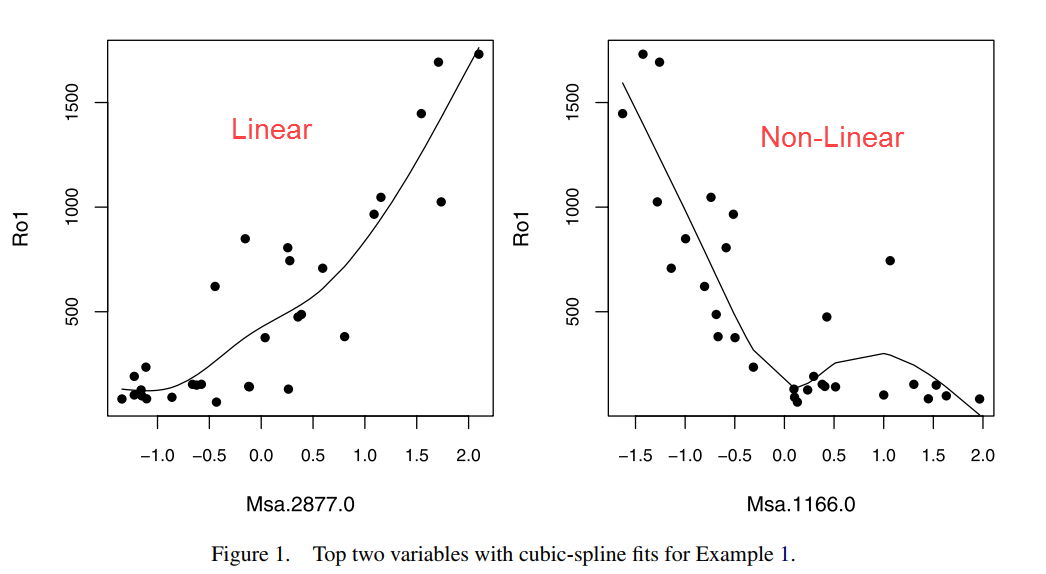
\includegraphics[width=0.90000\textwidth]{../figure/overlooking.png}
\end{center}

 
\section{Solution}
\subsection{Generalized Correlation}

\textit{\textbf{Generalized Correlation}}: In this paper, the authors introduce the generalized correlation, which extend the method for measuring non-linear relation. Let $\mathcal{H}$ denote a vector space of functions, which for simplicity we take to include all linear functions. Generally we could take $\mathcal{H}$ to be the vector space generated by any given set of functions h. Following is the simplified version of the Generalized Correlation. 

\begin{align*} 
      \psi_j &= \sup\limits_{h \in \mathcal{H}} \frac{cov\{h(X_{ij}), Y_i\}}{\sqrt{var\{h(X_{ij})\}}} \\   
      \hat{\psi}_j &= \sup\limits_{h \in \mathcal{H}} \frac{\sum_i\{h(X_{ij}) - \bar{h}\}(Y_i - \bar{Y})}{\sqrt{\sum_i \{h(X_{ij})-\bar{h}\}^2}}
\end{align*}


\textit{\textbf{Further simplified the computation (Theorem 1)}}: Assume $\mathcal{H}$ is a finite-dimensional function space include the constant function, and there exists $ h\in\mathcal{H}$ that achieves $\hat{\psi}_j$,

\[
\argmin{h \in \mathcal{H}} \sum^n\limits_{i = 1}\{Y_i - h(X_{ij})\}^2 \subseteq \argmax{h \in \mathcal{H}} \hat{\psi}_j
\]

The maximizer of $\hat{\psi}_j$ is the solution to least squares problem in $\mathcal{H}$

The benefit of transferring the problem into a least squares problem is that has an explicit analytic solution. This avoids a potentially cumbersome optimization problem and allows “basis expansions” of $X_{ij}$.

\textit{\textbf{Reduction of $\hat{\psi}_j$ in the size of squared error}}:
One implement of the theorem 1 is to change the generalized correlation into the size of the squared error.
\[
  \hat{\varphi}_j = \sum^n\limits_{i = 1} (Y_i - \bar{Y})^2 - \inf\limits_{h \in \mathcal{H}}\sum^n\limits_{i = 1}\{Y_i - h(X_{ij})\}^2
\]
Since $\hat{\varphi}_j$ keeps the relative relation of $\hat{\psi}_j$, we can use $\hat{\varphi}_j$'s for ranking.


\textit{\textbf{Ranking the Generalized Correlation}}: We order estimator $\hat{\psi}_j$ as $\hat{\psi}_{\hat{j}_1} \geq \dots \geq \hat{\psi}_{\hat{j}_p}$
 \[ \hat{j}_1 \succeq \dots \succeq \hat{j}_p\]
  $j \succeq j' means \hat{\psi}_j \geq \hat{\psi}_{j'}$, we could
  say jth coefficient of X is at least as much importance as the j'th
  coefficient
  $r = \hat{r}(j)$ means the rank of the jth coefficient is r, in
  other words $\hat{j}_r = j$
We could use Bootstrap to assess the empirical rank for each component
of X. A $(1-\alpha)$ level, two-side interval is defined as following: Interval of rank $[\hat{r}_{-}(j), \hat{r}_{+}(j)]$
\[
  P\{r^*(j)\leq \hat{r}_{-}(j)|\mathcal{D}\} \approx P\{r^*(j)\geq \hat{r}_{+}(j)|\mathcal{D}\} \approx \frac{\alpha}{2}
\]
 where, $r^*(j)$ the bootstrap version estimators of $r(j)$. The approximation is used because of the discreteness of ranks. Small value of $r^*(j)$ indicates large influence on Y. In order to select variables, we could sort $r^*(j)$ or $\hat{r}_{+}(j)$ and set a cut off value $p$.
 
\section{Simulation result}
\subsection{Setting up}

\begin{itemize}
\item $W_i \sim Unif[-2,2]$
\item
  $X_{i1} = W_{i} + \delta_i$ (errors-in-variables type)
\item
  $X_{i2}, \dots, X_{i5000} \stackrel{iid}{\sim} N(0,1)$
\item
  $\delta, \epsilon \stackrel{iid}{\sim} N(0, 3/4)$
\item
  $n = 200, ~ \alpha = 0.02, n_{times ~of ~bootstrap} = 500$
\end{itemize}
\subsection{result}

\begin{center}

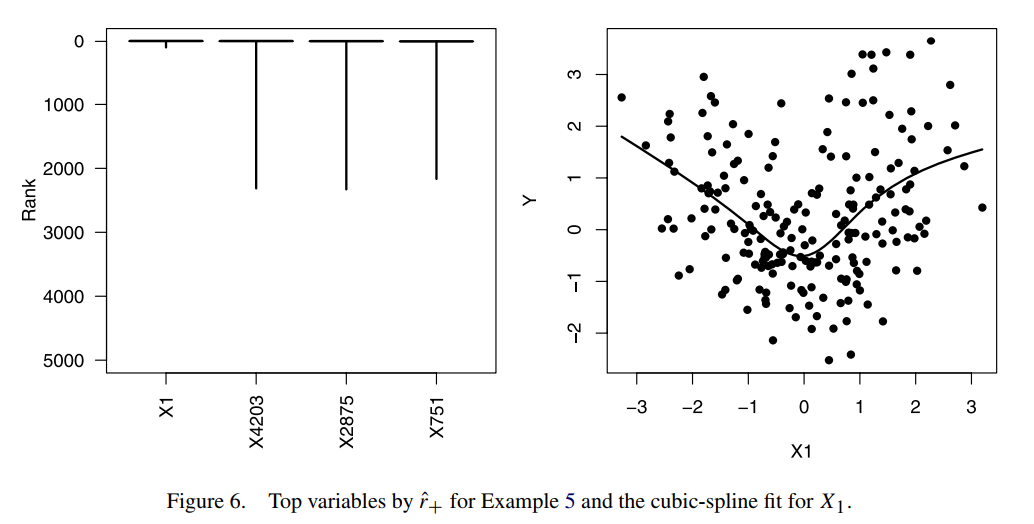
\includegraphics[width=0.70000\textwidth]{../figure/sim_non_linear.png}

\end{center}

The cutoff value for choose the important variable is $p/2$. From the figure above you can see that the conventional correlation fails to select $X_{i1}$ as influential variable Generalized correlation method is able to select the $X_{i1}$ with only 3 false positive variables.


\begin{thebibliography}{9}

\bibitem{r1}
\textsc{Peter HALL, Hugh MILLER.} (2009). \textit{Using Generalized Correlation to Effect Variable Selection in Very High Dimensional Problems.'}

\end{thebibliography}

\end{document}